\pdftrailerid{}
\newcommand{\DoNotLoadEpstopdf}{}
\documentclass[11pt]{article}
\usepackage[T1]{fontenc}
\usepackage{lmodern}
\usepackage[margin=1in]{geometry}
\usepackage{amsmath,amssymb,amsthm,mathtools}
\usepackage{microtype}
\usepackage{enumitem}
\usepackage{tikz}
\usetikzlibrary{arrows.meta,positioning,calc}
\usepackage{xcolor}
\definecolor{linkblue}{RGB}{25,65,105}
\usepackage[colorlinks=true,allcolors=linkblue,breaklinks=true]{hyperref}
\usepackage{bookmark}
\usepackage[nameinlink,noabbrev]{cleveref}
\hypersetup{pdftitle={Critical bond and site percolation on the cubic lattice},pdfauthor={OpenAI}}
\newtheorem{theorem}{Theorem}[section]
\newtheorem{lemma}[theorem]{Lemma}
\newtheorem{proposition}[theorem]{Proposition}
\newtheorem{corollary}[theorem]{Corollary}
\theoremstyle{definition}
\newtheorem{definition}[theorem]{Definition}
\theoremstyle{remark}
\newtheorem{remark}[theorem]{Remark}
\numberwithin{equation}{section}
\setlist[itemize]{leftmargin=*,itemsep=3pt,topsep=5pt}
\setlist[enumerate]{leftmargin=*,itemsep=3pt,topsep=5pt}
\setlength{\emergencystretch}{2em}
\title{Critical bond and site percolation on the cubic lattice}
\author{OpenAI}
\date{September 24, 2026}
\begin{document}
\maketitle
\begin{abstract}
We prove that nearest-neighbor Bernoulli bond and site percolation on
$\mathbb Z^3$ have no infinite cluster at their respective critical parameters.
The proof combines a finite connection inequality for independent hyperedges
with a finite-scale extension estimate and an adaptive exploration.
\end{abstract}
\section{Introduction}

In Bernoulli bond percolation on the nearest-neighbor cubic lattice
$\mathbb Z^3$, each edge is independently open with probability $p$.
In Bernoulli site percolation, the independent open bits instead belong to
the vertices, and an open path must have every vertex open, including its
endpoints. Write $\mathbb P_p$ for the law of the model under consideration
and define its critical parameter by
\[
 p_c=\inf\{p\in[0,1]:
       \mathbb P_p(0\text{ belongs to an infinite open cluster})>0\}.
\]
By translation invariance and a countable union over vertices, the same
threshold is obtained by asking for the existence of any infinite cluster.
The bond and site thresholds are defined separately throughout.

\begin{theorem}\label{thm:main}
For nearest-neighbor Bernoulli bond percolation on $\mathbb Z^3$, there is
almost surely no infinite open cluster at the bond critical parameter.
The same assertion holds for nearest-neighbor Bernoulli site percolation
at the site critical parameter.
\end{theorem}

Write $\theta(p)=\mathbb P_p(0\text{ belongs to an infinite open cluster})$.
The theorem gives continuity at the transition: $\theta(p)$ tends to
zero as $p\downarrow p_c$. To see this consequence directly, for $n\ge1$ let $E_n$ be
the event that the origin reaches the boundary of the box
$[-n,n]^3\cap\mathbb Z^3$ by an open path inside that box. Then
$\mathbb P_p(E_n)\downarrow\theta(p)$ as $n\to\infty$. At $p_c$, the
theorem makes this limit zero. Given $\varepsilon>0$, first choose $n$
with $\mathbb P_{p_c}(E_n)<\varepsilon$; since $E_n$ depends on finitely
many bits, the same strict inequality holds for $p$ sufficiently close
to $p_c$. Thus $\theta(p)\le\mathbb P_p(E_n)<\varepsilon$ there.
The proof below establishes critical extinction for both models without
using an external criticality theorem.

\paragraph{History and the three-dimensional obstacle.}
Broadbent and Hammersley introduced percolation to study transport through
a random medium~\cite{BroadbentHammersley1957}. In two dimensions, Harris's
critical nonpercolation theorem and Kesten's identification of the square
bond threshold established the bond result~\cite{Harris1960,Kesten1980}.
Russo proved critical nonpercolation for nearest-neighbor site percolation
on the square lattice~\cite[Theorem~2(b)]{Russo1981}. These planar results
use geometry that is unavailable for paths in three dimensions.

In sufficiently high dimensions, Hara and Slade established mean-field
critical behavior through the lace expansion~\cite{HaraSlade1990}.
Fitzner and van der Hofstad obtained the nearest-neighbor bond range
$d\ge11$~\cite{FitznerHofstad2017}. Hara and Slade also noted that their method applies to site
percolation~\cite[p.~335]{HaraSlade1990}. Heydenreich and Matzke later gave
a detailed site lace-expansion treatment, proving the triangle condition
in sufficiently high dimensions and its critical nonpercolation
consequence~\cite[Theorem~1.1 and Section~1.3]{HeydenreichMatzke2020}. The explicit bond dimension bound is
not a site bound. Benjamini and Schramm formulated the broader criticality
question for quasi-transitive graphs with $p_c<1$~\cite[Conjecture~4]{BenjaminiSchramm1996}.

Grimmett and Marstrand proved convergence of slab thresholds to the
full-lattice threshold and developed a dynamic renormalization argument
using open seeds and sequentially controlled exploration~\cite{GrimmettMarstrand1990}.
Duminil-Copin, Sidoravicius, and Tassion subsequently proved critical
nonpercolation for bond percolation on slabs~\cite{DuminilCopinSidoraviciusTassion2016}.
As their discussion explains, extinction at every fixed slab threshold,
together with convergence of those thresholds, does not by itself give
critical extinction in the full cubic lattice. The proof here obtains the
required connections between finite regions from a finite comparison,
and fixes all scales before decreasing the percolation parameter.

Leder's public account of a Lean formalization reports critical bond
nonpercolation on every nearest-neighbor lattice $\mathbb Z^d$,
$d\ge2$~\cite{Leder2026}. Its first-contact comparison
\cite[Section~3.4, (GEN)]{Leder2026} already implies the finite joint connection inequality for
bonds: take the increasing cluster functional to indicate meeting the
target set. The subsequent public Kozma--Nitzan exposition explicitly
records this consequence and reports stronger finite
comparisons~\cite[``Conjecture~1 from the Lean proof of Conjecture~3'']{KNPublic2026}.
The related public site exposition reports the
independent labelled-hyperedge comparison, a conditioned-covariance
hierarchy, and critical site nonpercolation on $\mathbb Z^d$ for every
$d\ge3$~\cite[``One inequality for both models'',
``Conditional covariance inequalities'', and ``From (1) to the lattice'']{SitePublic2026}.
These two public expositions describe work produced by AI systems
prompted by Ahmed Bou-Rabee. Our purpose here is a
self-contained cubic argument, including the finite comparison, explicit
relay geometry, and exploration estimates.

\paragraph{Finite comparison and the proof method.}
Our main finite ingredient is a connection inequality for independent,
possibly nonuniform hyperedges. For a node $o$ and nonempty node set $A$,
it asserts that
\begin{equation}\label{intro:comparison}
 \mathbb P(o\leftrightarrow A,\ o\leftrightarrow T)
 \ge \mathbb P(o\leftrightarrow A)
          \min_{a\in A}\mathbb P(a\leftrightarrow T).
\end{equation}
Here an open hyperedge joins all of its nodes. The inequality implies that
if every possible relay in $A$ reaches a target $T$ with probability at
least $1-b$, then the probability of reaching $A$ but missing $T$ is at
most $b$. This failure bound also holds for sites, and after any set of bits
has been fixed while the remaining bits retain their product law. Thus it
remains available during an exploration.

Taking $T$ to be a singleton in \eqref{intro:comparison} and enlarging
the event on the left gives the multiplicative gluing inequality of
Kozma and Nitzan~\cite[Conjecture~1]{KozmaNitzan2024}.
They also record that van den Berg and Engelenburg independently
considered this inequality. Section~4 of Kozma and Nitzan connects finite comparisons
to criticality through renormalization. The proof of
\eqref{intro:comparison} uses increasing functions of clusters, a
nonnegative cone of conditional connection columns, and alternating
conditional cluster resampling. Conditional resampling has precedents in
percolation correlation inequalities \cite[Section~2.1]{BHK2006}.
We prove the required comparison and every lattice relay estimate locally.
The general bond criticality theorem does not imply the site assertion:
independent site bits become independent hyperedges, and their endpoint
convention must be preserved. The finite hyperedge comparison
and its stability under fixed bits are useful independently of the lattice
application.

\paragraph{Proof overview.}
Assume that an infinite cluster exists at $p_c$. Large seed boxes then
connect with high probability to each of the 24 quarter-faces of a surrounding
cube. Only finitely many radii are needed, so these estimates persist at one
parameter $q<p_c$.

The finite comparison lets us extend a connection through a fresh region.
The seed and sequential-exploration architecture is related to the dynamic
renormalization method of Grimmett and Marstrand~\cite[Sections~3--4]{GrimmettMarstrand1990}.
Here many well-separated entrance points provide independent chances for an
open seed, while relay quality is defined using the interior bits alone. A
sequence of thirteen elementary geometric moves transfers a connection from
the inner box of one coarse cube to that of its neighbor. Finally, we explore
cubes indexed by $\mathbb Z^2$, retaining a high conditional connection
probability for each pending cube. Each processed cube has a uniformly small
conditional chance of failure. A planar boundary count then gives a positive
chance of infinitely many successful cubes, and hence an infinite open
cluster at $q<p_c$, a contradiction. Neither uniqueness of the infinite
cluster nor independence of the successful coarse cubes is assumed.

Section~\ref{sec:comparison} proves the finite comparison.
Section~\ref{sec:preliminaries} gives the planar count and fixes the scales.
Sections~\ref{sec:extension} and~\ref{sec:geometry} prove the extension
and neighboring-box estimates. Section~\ref{sec:exploration} constructs
the exploration and completes the proof.

\paragraph{Connection conventions.}
For a vertex $x$ and vertex set $T$, the notation $x\leftrightarrow T$
means that an open path in the specified graph joins $x$ to some vertex of
$T$. For two sets, at least one pair of their vertices must be so joined.
We permit paths of zero edges. Such a path always gives a self-connection
for bonds and hyperedges, but for sites its single vertex must be open.
All graphs and hypergraphs in the finite comparison are undirected.

\section{A finite connection comparison}\label{sec:comparison}

The lattice argument will need to pass from a connection to a set of possible
relays to a connection to a target. We prove the finite inequality that makes
this passage possible, allowing different probabilities for the independent
bits so that the result remains available after some bits have been fixed.

A finite hypergraph has a finite node set and a finite labelled family of
nonempty subsets called hyperedges; distinct labels may represent the same
subset. Each hyperedge is independently open with its own probability; an
open hyperedge joins all its nodes. The cluster $C(x)$ always
contains $x$, and $C(S)=\bigcup_{x\in S}C(x)$. All connections in this section
are in finite undirected graphs or hypergraphs.

\begin{proposition}[Joint connection comparison]\label{cmp:joint}
In independent percolation on a finite hypergraph, with arbitrary hyperedge
probabilities in $[0,1]$, let $o$ be a node and let $A,T$ be node sets with
$A\ne\varnothing$. Then
\begin{equation}\label{cmp:joint-bound}
 \mathbb P(o\leftrightarrow A,\ o\leftrightarrow T)
 \ge \mathbb P(o\leftrightarrow A)
       \min_{a\in A}\mathbb P(a\leftrightarrow T).
\end{equation}
\end{proposition}

For bonds, subtraction immediately turns this inequality into the failure
bound needed later. Sites require an additional check because a hypergraph
node is always connected to itself, whereas a site self-connection requires
an open vertex. We give that check at the end of the section.

The proof of Proposition~\ref{cmp:joint} assigns each cluster meeting an
ordered list to its first node in that list. Conditional connection probabilities form the columns
of a triangular matrix. The positivity property below will bound the source's
joint connection probability from below by a nonnegative weighted sum of relay-to-target
probabilities. The weights will total the probability of reaching the relay
set, giving the proposition.

Deleting a node set $w$ means deleting its nodes and every hyperedge meeting
it; write $G\setminus w$ for the resulting hypergraph. On an exact-cluster
event $C(S)=w$ of positive probability, the hyperedges of $G\setminus w$
retain their independent original laws. Indeed, the event asks that every
node of $w$ connect to $S$ within $w$, and that all hyperedges crossing from
$w$ to its complement be closed. It tests no hyperedge disjoint from $w$.
The same observation applies after an earlier deletion.

\begin{lemma}[Cluster columns]\label{cmp:cone}
Let $G$ be a finite hypergraph whose hyperedges have independent open
probabilities strictly less than one.
Choose any ordered list of distinct nodes $x_1,\ldots,x_n$; the list need
not contain every node. Define
\[
 S_k=\{x_i:i<k\},\qquad
 E_k=\{C(x_k)\cap S_k=\varnothing\},\qquad
 d_k=\mathbb P(E_k)>0,
\]
and let $\mu_k$ be the conditional law of $C(x_k)$ given $E_k$, regarded
as a measure on
\[
 \mathcal D_k=\{U:x_k\in U,\ U\cap S_k=\varnothing\}.
\]
For a function $F$ on $\mathcal D_k$, let
\[
 v_k^F(i)=\mathbb E_{\mu_k}
       [\mathbf 1_{\{x_i\in U\}}F(U)],\qquad
 h_k=v_k^1,\qquad H=(h_1\ \cdots\ h_n).
\]
If $F$ is nonnegative and increasing under inclusion, then
\begin{equation}\label{cmp:cone-relation}
 v_k^F-\mu_k(F)h_k
   \in\operatorname{cone}\{h_j:k<j\le n\}.
\end{equation}
Here the cone consists of all nonnegative linear combinations, including
zero. In particular, $H^{-1}v_k^F$ is coordinatewise nonnegative.
\end{lemma}

\begin{proof}
Closing every hyperedge incident to $x_k$ proves $d_k>0$. The matrix $H$
is unit lower triangular: its $k$th column vanishes above row $k$ and has
entry one in row $k$. We prove \eqref{cmp:cone-relation} by descending
induction on $k$. For $k=n$, both $v_n^F$ and $\mu_n(F)h_n$ equal
$\mu_n(F)e_n$, where $e_n$ is the $n$th coordinate vector.

Fix $k<n$ and assume the assertion for every later column. Write
$s=x_k$, $S=S_k$, and $W=C(S)$. For a set $w\supseteq S$ avoiding $s$, put
\[
 c(w)=\mathbb E\bigl[F(C^{G\setminus w}(s))\bigr],
\]
where the expectation uses the original product law on the undeleted
hyperedges. Restriction of the same configuration shows that $c(w)$ is
nonincreasing in $w$.

\paragraph{A first-listed-node decomposition.}
Fix a row $i$. For $j>k$, let $L_{ij}$ be the event that the first listed
node of $C(x_i)$ is $x_j$.
Condition on an exact value $W=w$ avoiding $s$. Then the mean of $F(C(s))$
is $c(w)$. If $x_i\notin w$, its cluster contains the listed node $x_i$
and avoids all listed nodes preceding $s$, which belong to $w$.
Its first listed node is therefore $s$ precisely when $x_i\in C(s)$;
otherwise exactly one of the events $L_{ij}$ occurs.
On $L_{ij}$, condition further on $C(x_j)=U$. The set $U$ avoids $s$, and
the specification of $L_{ij}$ adds only membership and avoidance conditions
on $U$. Exact-cluster conditioning therefore leaves the mean of $F(C(s))$
equal to $c(w\cup U)$. Partitioning the expectation $c(w)$ and subtracting
$c(w)$ times the corresponding partition of total probability gives
\begin{align}
 &\mathbb E[\mathbf 1_{\{x_i\in C(s)\}}F(C(s))\mid W=w]
 \notag\\
 &\quad=c(w)\mathbb P(x_i\in C(s)\mid W=w)
   +\sum_{j>k}\mathbb E\bigl[
       \mathbf 1_{L_{ij}}\{c(w)-c(w\cup C(x_j))\}\mid W=w\bigr].
 \label{cmp:partition}
\end{align}
The expressions involving $c(w\cup C(x_j))$ are evaluated only on
$L_{ij}$. If $x_i\in w$, all $L_{ij}$ are empty under the conditioning,
and both sides vanish.

For $U$ disjoint from $S$, let
$W_U=C^{G\setminus U}(S)$. Define, for $U\in\mathcal D_k$,
\[
 (PF)(U)=\mathbb E[c(W_U)],
\]
and, for $U$ disjoint from $S\cup\{s\}$, define
\begin{equation}\label{cmp:residual}
 R_F(U)=\mathbb E\bigl[
   \mathbf 1_{\{s\notin W_U\}}
   \{c(W_U)-c(W_U\cup U)\}\bigr],
\end{equation}
with zero integrand when $s\in W_U$. The operator $P$ preserves
nonnegativity and monotonicity: enlarging $U$ shrinks $W_U$, whereas $c$
is nonincreasing.

We now average \eqref{cmp:partition} conditional on $E_k$. Given
$C(s)=U$ avoiding $S$, the conditional law of $W$ is that of $W_U$.
Thus the first term on the right averages to
\[
 \mathbb E_{\mu_k}[\mathbf 1_{\{x_i\in U\}}(PF)(U)]
 =v_k^{PF}(i).
\]
For a residual term, the exact event identity is
\[
 E_k\cap L_{ij}
 =E_k\cap E_j\cap\{x_i\in C(x_j)\}.
\]
Indeed, a cluster avoiding the earlier listed nodes also avoids their entire
clusters. Given $C(x_j)=U$ under $E_j$, the conditional law of $W$ is again
that of $W_U$, and the remaining restriction $E_k$ is $s\notin W_U$.
Consequently the unnormalized residual expectation is
\[
 \mathbb E\!\left[
  \mathbf 1_{E_k\cap L_{ij}}
   \{c(W)-c(W\cup C(x_j))\}\right]
 =d_j\,\mathbb E_{\mu_j}
       [\mathbf 1_{\{x_i\in U\}}R_F(U)],
\]
where the expression on the left is evaluated only when its indicator is one.
Dividing by $d_k$ and summing over $j>k$ proves the column identity
\begin{equation}\label{cmp:column-identity}
 v_k^F=v_k^{PF}+\sum_{j>k}\frac{d_j}{d_k}v_j^{R_F}.
\end{equation}
Here and below $R_F$ is restricted to $\mathcal D_j$ in the $j$th column.
To complete the induction, we show that $R_F$ is nonnegative and increasing
and that $P^tF$ converges uniformly to $\mu_k(F)$.

\paragraph{The residual is increasing.}
Sample all hyperedge bits once, and use their restrictions after every
deletion. For deterministic $U$ disjoint from $S\cup\{s\}$, the event
$W_U=w$ tests only bits of hyperedges disjoint from $U$ and meeting $w$.
Every full-graph hyperedge disjoint from $w$ therefore retains its independent
original law after this conditioning, including hyperedges that meet $U$.
When $s\notin w$, the two clusters in the following difference consequently
have the marginal laws defining $c(w)$ and $c(w\cup U)$.
Hence $R_F(U)=\mathbb E[D_U]$, where
\begin{equation}\label{cmp:residual-sample}
 D_U=\mathbf 1_{\{s\notin W_U\}}
 \left\{F(C^{G\setminus W_U}(s))
       -F(C^{G\setminus(W_U\cup U)}(s))\right\},
\end{equation}
again interpreted as zero on the excluded event. All clusters at which
$F$ is evaluated contain $s$ and avoid $S$.

The first cluster contains the second, so $D_U\ge0$. To compare two sets
$U\subseteq U'$, first note that $W_{U'}\subseteq W_U$. On
$\{s\notin W_U\}$, deleting the smaller set $W_{U'}$ makes the first
cluster larger. The second cluster has a different monotonicity:
\[
 C^{G\setminus(W_U\cup U)}(s)=C^{G\setminus U}(s).
\]
Indeed, in $G\setminus U$ the source cluster is disjoint from the union
$W_U$ of the $S$-clusters, so deleting $W_U$ removes none of its open
connections. The same equality holds for $U'$, because $s\notin W_{U'}$.
Thus the second cluster becomes smaller when $U$ is replaced by $U'$.
Both changes increase the difference of the two values of $F$, giving
$D_{U'}\ge D_U$. On $\{s\in W_U\}$, this inequality follows instead from
$D_U=0$ and $D_{U'}\ge0$. Taking expectations proves that $R_F$ is
nonnegative and increasing.

\paragraph{Conditional resampling and the limit.}
The operator $P$ is a Markov transition: from $U$, first sample $W_U$, then
independently sample $C^{G\setminus W_U}(s)$. Under the joint law of
$(C(s),W)$ conditional on $E_k$, these are the successive conditional laws
of $W$ given $C(s)$ and of $C(s)$ given $W$. Hence $\mu_k$ is stationary
for $P$. Alternating conditional cluster resampling under a separation
condition is the method used by van den Berg, H\"aggstr\"om, and
Kahn~\cite[Section~2.1, proof of Theorem~2.1]{BHK2006}; the cone conclusion here is proved by
the following iteration.

Every transition assigns probability at least
\[
 a=\prod_{e:\,s\in e}(1-p_e)>0
\]
to the singleton $\{s\}$, since closing every incident hyperedge suffices
to isolate $s$ in any deletion graph. Thus, for every real function $g$ on
the finite state space $\mathcal D_k$, subtracting this common mass gives
\[
 \max Pg-\min Pg\le(1-a)(\max g-\min g).
\]
Iteration makes the oscillation of $P^tF$ tend to zero. Its $\mu_k$-mean
remains $\mu_k(F)$ by stationarity, so
\[
 \sup_{U\in\mathcal D_k}|(P^tF)(U)-\mu_k(F)|
 \le(1-a)^t(\max F-\min F)\longrightarrow0.
\]
This proves the required uniform convergence, including at states of
$\mathcal D_k$ with zero $\mu_k$-mass.

By the induction hypothesis, each $v_j^{R_F}$ is a nonnegative combination
of $h_j,\ldots,h_n$. Equation~\eqref{cmp:column-identity} therefore puts
$v_k^F-v_k^{PF}$ in the cone on the right of
\eqref{cmp:cone-relation}. All iterates $P^tF$ remain nonnegative increasing,
so iteration puts $v_k^F-v_k^{P^tF}$ in that cone as well. The cone is closed,
because its generators belong to the basis given by the columns of $H$.
Taking the uniform limit proves \eqref{cmp:cone-relation}. Finally, adding
$\mu_k(F)h_k$ expresses $v_k^F$ as a nonnegative combination of columns of
$H$, proving the last assertion.
\end{proof}

\begin{proof}[Proof of Proposition~\ref{cmp:joint}]
First suppose all probabilities are below one. Use the notation of
Lemma~\ref{cmp:cone}. For
$F(U)=\mathbf 1_{\{x_j\in U\text{ for some }j>k\}}$, isolation of $x_k$
gives $\mu_k(F)<1$, and direct inspection of the rows gives
\[
 v_k^F-\mu_k(F)h_k=(1-\mu_k(F))(h_k-e_k),
\]
where $e_k$ is the $k$th coordinate vector. Lemma~\ref{cmp:cone} yields
nonnegative coefficients $\Gamma_{jk}$ such that
\[
 h_k=e_k+\sum_{j>k}\Gamma_{jk}h_j.
\]
With $\Gamma$ zero on and above the diagonal, these column identities say
$H=I+H\Gamma$, or $H^{-1}=I-\Gamma$. Also, for $d=(d_1,\ldots,d_n)^\mathsf T$,
\begin{equation}\label{cmp:first-node-mass}
 Hd=\mathbf 1,\qquad (I-\Gamma)\mathbf 1=d.
\end{equation}
Indeed, the cluster of $x_i$ has first listed node $x_k$ with probability
$d_kh_k(i)$, and these events partition the sample space.

If $o\in A$, \eqref{cmp:joint-bound} is immediate. Otherwise take the list
to consist exactly of the nodes of $A$, in any order, followed by $x_n=o$.
Set
\[
 F(U)=\mathbf 1_{\{U\cap A\ne\varnothing,\ U\cap T\ne\varnothing\}},
 \qquad y_i=\mathbb E[F(C(x_i))].
\]
Partitioning by the first listed node gives
$y=\sum_k d_kv_k^F$, where $F$ is restricted to $\mathcal D_k$ in each
summand. Every restriction is nonnegative increasing, so
Lemma~\ref{cmp:cone} gives $(I-\Gamma)y\ge0$ coordinatewise. In the last row,
\[
 y_n\ge\sum_{i<n}\Gamma_{ni}y_i.
\]
For $i<n$, $y_i=\mathbb P(x_i\leftrightarrow T)$, while
$y_n=\mathbb P(o\leftrightarrow A,\ o\leftrightarrow T)$. By
\eqref{cmp:first-node-mass}, the nonnegative weights in this row sum to
\[
 \sum_{i<n}\Gamma_{ni}=1-d_n=\mathbb P(o\leftrightarrow A).
\]
This proves \eqref{cmp:joint-bound}. Finally, finite event probabilities are
polynomials in the hyperedge parameters, and the minimum in
\eqref{cmp:joint-bound} is finite. Continuity therefore allows probabilities
equal to one as well.
\end{proof}

\begin{corollary}[Failure comparison]\label{cmp:failure}
Consider independent bond or site percolation on a finite undirected graph,
with arbitrary individual probabilities in $[0,1]$. For a vertex $o$, vertex
sets $A,T$, and $b\in[0,1]$, if
\[
 \mathbb P(a\leftrightarrow T)\ge1-b\qquad(a\in A),
\]
then
\begin{equation}\label{cmp:failure-bound}
 \mathbb P(o\leftrightarrow A,\ o\not\leftrightarrow T)\le b.
\end{equation}
The assertion therefore applies after any deterministic collection of bits
has been fixed.
\end{corollary}

\begin{proof}
The empty-set case $A=\varnothing$ is immediate. For bonds,
Proposition~\ref{cmp:joint} and subtraction give the stronger upper bound
$b\mathbb P(o\leftrightarrow A)\le b$.

For sites, use the incidence construction described
in~\cite[``One inequality for both models'']{SitePublic2026}.
Create a node $x^*$ for every graph vertex $x$ and a connector node for every
graph edge. For each site $x$, form a hyperedge consisting
of $x^*$ and all connector nodes corresponding to edges incident to $x$;
its independent open bit is the bit of site $x$. For distinct vertices
$x,z$, connection of $x^*$ to $z^*$ is equivalent to an open site path
from $x$ to $z$. Hypergraph self-connection, however, always holds.
Writing $A^*,T^*$ for the starred images, we consequently have
\[
 \mathbb P_{\mathrm{hyp}}(a^*\leftrightarrow T^*)
 \ge\mathbb P_{\mathrm{site}}(a\leftrightarrow T)\ge1-b.
\]
On the site event in \eqref{cmp:failure-bound}, the origin $o$ is open.
Its hypergraph connections to starred vertices therefore agree with its
site connections, including a possible zero-edge path to itself. This gives
the event inclusion
\[
 \{o\leftrightarrow A,\ o\not\leftrightarrow T\}_{\mathrm{site}}
 \subseteq
 \{o^*\leftrightarrow A^*,\ o^*\not\leftrightarrow T^*\}_{\mathrm{hyp}}.
\]
Applying Proposition~\ref{cmp:joint} and subtraction to the hypergraph bounds
the latter event by $b$, proving the site assertion. Fixed bits are exactly
parameters equal to zero or one, already allowed in the statement.
\end{proof}

\section{Planar boundaries and finite scales}\label{sec:preliminaries}

We now fix either the bond or the site model. This section supplies a planar
boundary count and chooses all the finite scales needed to lower the parameter.
The boundary count will be used first to show $p_c<1$, and then to prove that
the adaptive exploration survives.

\subsection{A deterministic boundary count}

An edge of the dual square lattice
$\mathbb Z^2+(1/2,1/2)$ crosses exactly one primal edge of $\mathbb Z^2$.
For a finite set $X\subset\mathbb Z^2$, its dual edge boundary consists of
the dual edges crossing primal edges with exactly one endpoint in $X$.

\begin{lemma}[Boundary cycles]\label{prelim:contours}
There are deterministic families $\mathcal C_n$ of simple dual cycles of
length $n$, with $|\mathcal C_n|\le 2n3^n$, such that the dual edge boundary
of every finite $X\subset\mathbb Z^2$ containing $0$ includes a cycle in
$\bigcup_{n\ge1}\mathcal C_n$. For each cycle in $\mathcal C_n$, one can
fix at least $n/7$ of its crossed primal edges with pairwise disjoint endpoints.
\end{lemma}

\begin{proof}
At a dual vertex, the boundary degree counts the membership changes around
a primal square, and is therefore even. The finite dual boundary consequently
decomposes into edge-disjoint simple cycles: extract a simple cycle whenever
an edge remains, and remove its edges, preserving even degrees.

Along the positive horizontal ray from $0$, the total number of boundary
crossings is odd, since membership in $X$ starts at one and eventually becomes
zero. At least one cycle in the decomposition has an odd number of positive-ray
crossings. The total number of crossings of a closed dual cycle with the whole
horizontal line is even, by counting changes of the sign of the height.
The selected cycle therefore also crosses the negative ray.

If its length is $n$, a positive crossing has horizontal coordinate
$t+1/2$ for some integer $0\le t<n$: the horizontal distance to a negative
crossing is less than $n$. Define $\mathcal C_n$ to be all simple length-$n$
cycles having such an anchored crossing and an odd number of positive-ray
crossings. There are at most $n$ choices for the anchored edge, two orientations,
and at most $3^n$ nonbacktracking continuations. This proves the asserted
overcount. Finally, greedily select crossed primal edges in a fixed order,
discarding all edges incident to either endpoint of each selection. Each
selection discards at most seven edges, including itself, because the primal
degree is four. The selected edges have disjoint endpoints and number at least
$n/7$.
\end{proof}

\begin{lemma}\label{prelim:pc-below-one}
For both models on $\mathbb Z^3$, $p_c<1$.
\end{lemma}

\begin{proof}
It suffices to percolate on a coordinate copy of $\mathbb Z^2$. In the bond
model, if the origin cluster there is finite, all primal edges crossed by its
dual boundary are closed. Lemma~\ref{prelim:contours} and a union bound give
\[
 \mathbb P_p(0\text{ has a finite planar cluster})
 \le \sum_{n\ge1}2n3^n(1-p)^n<1
\]
for $p<1$ sufficiently close to one.

For sites, first separate the event that $0$ is closed. If its open planar
cluster is finite, each edge crossed by the boundary cycle has a closed
endpoint. For a fixed candidate cycle, select $k\ge n/7$ edges with disjoint
endpoints as in Lemma~\ref{prelim:contours}. The union over choices of one
closed endpoint of each edge has probability at most $[2(1-p)]^k$.
For $p$ close to one, $2(1-p)<1$, so
\[
 \mathbb P_p(0\text{ is not in an infinite planar open cluster})
 \le (1-p)+\sum_{n\ge1}2n3^n[2(1-p)]^{n/7}<1.
\]
Indeed both displayed series are convergent geometric-power series tending
to zero as $p\uparrow1$. This proves the lemma.
\end{proof}

\subsection{Seed boxes and quarter-faces}

For $u\in\mathbb Z^3$ and a nonnegative integer $b$, write
\[
 \Lambda_b(u)=u+([-b,b]^3\cap\mathbb Z^3),\qquad \Lambda_b=\Lambda_b(0).
\]
A \emph{quarter-face} of $\Lambda_b(u)$ is obtained by setting one coordinate
relative to $u$ equal to $b$ or $-b$, and restricting each remaining coordinate
to either $[0,b]$ or $[-b,0]$. There are 24 such quarter-faces; overlaps on their
boundaries do not matter. More explicitly, for a normal index
$i\in\{1,2,3\}$, a sign $\sigma\in\{-1,+1\}$, and signs
$\varepsilon_j\in\{-1,+1\}$ for the two indices $j\ne i$, set
\begin{equation}\label{prelim:face-index}
 F_{i,\sigma}^{(\varepsilon_j)_{j\ne i}}(u,b)
 =\{u+x:x_i=\sigma b,\quad
                  0\le\varepsilon_jx_j\le b\ (j\ne i)\}.
\end{equation}
The six choices of $(i,\sigma)$ and the four choices of the transverse
sign pair enumerate all 24 faces. Figure~\ref{prelim:quarterfaces-figure}
illustrates this indexing.
A bit is \emph{internal} to a vertex set if it is a
site in that set, or, for bonds, an edge with both endpoints in that set.

\begin{figure}[tbp]
\centering
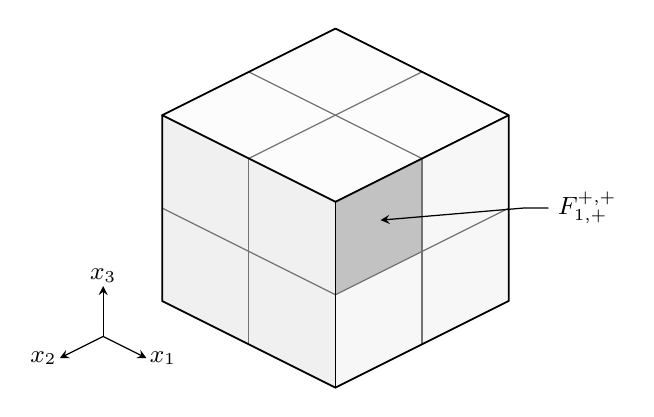
\begin{tikzpicture}[
  x={(1.10cm,-0.55cm)},
  y={(-1.10cm,-0.55cm)},
  z={(0cm,1.18cm)},
  font=\small,
  line join=round,
  line cap=round,
  >=stealth,
  qf edge/.style={black,line width=0.65pt},
  qf division/.style={black!55,line width=0.45pt}
]
  \fill[black!3] (1,-1,-1)--(1,1,-1)--(1,1,1)--(1,-1,1)--cycle;
  \fill[black!6] (-1,1,-1)--(1,1,-1)--(1,1,1)--(-1,1,1)--cycle;
  \fill[black!1] (-1,-1,1)--(1,-1,1)--(1,1,1)--(-1,1,1)--cycle;

  \fill[black!24] (1,0,0)--(1,1,0)--(1,1,1)--(1,0,1)--cycle;

  \draw[qf division] (1,0,-1)--(1,0,1);
  \draw[qf division] (1,-1,0)--(1,1,0);
  \draw[qf division] (0,1,-1)--(0,1,1);
  \draw[qf division] (-1,1,0)--(1,1,0);
  \draw[qf division] (0,-1,1)--(0,1,1);
  \draw[qf division] (-1,0,1)--(1,0,1);

  \draw[qf edge]
    (1,-1,-1)--(1,1,-1)--(-1,1,-1)--(-1,1,1)
    --(-1,-1,1)--(1,-1,1)--cycle;
  \draw[qf edge] (1,1,1)--(1,1,-1);
  \draw[qf edge] (1,1,1)--(-1,1,1);
  \draw[qf edge] (1,1,1)--(1,-1,1);

  \coordinate (qf representative) at (1,0.48,0.56);
  \begin{scope}[x=1cm,y=1cm]
    \node[anchor=west] (qf label) at (2.70,0.00) {$F_{1,+}^{+,+}$};
    \draw[->,line width=0.45pt]
      (qf label.west)--(2.38,0.00)--(qf representative);

    \coordinate (qf axes) at (-2.95,-1.63);
    \draw[->,line width=0.45pt]
      (qf axes)--(-2.40,-1.905) node[right,inner sep=1pt] {$x_1$};
    \draw[->,line width=0.45pt]
      (qf axes)--(-3.50,-1.905) node[left,inner sep=1pt] {$x_2$};
    \draw[->,line width=0.45pt]
      (qf axes)--(-2.95,-0.99) node[above,inner sep=1pt] {$x_3$};
  \end{scope}
\end{tikzpicture}
\caption{Quarter-faces of $\Lambda_b(u)$, shown schematically for $b>0$.
Each of the three visible faces is divided into four quarter-faces;
the three opposite faces are divided in the same way.
Thus $3$ normal axes $\times\,2$ normal signs $\times\,4$ transverse sign pairs
give $24$ quarter-faces. Boundary overlaps are permitted.
The shaded example $F_{1,+}^{+,+}$ has $x_1-u_1=b$ and
$0\le x_2-u_2,x_3-u_3\le b$.}
\label{prelim:quarterfaces-figure}

\end{figure}

Suppose, towards a contradiction, that at $p=p_c$ an infinite cluster exists
with positive probability. Then $0<p<1$ by Lemma~\ref{prelim:pc-below-one}
and the absence of percolation at zero. In fact an infinite cluster exists
almost surely. To see this without a uniqueness assumption, the existence event
is invariant under changing finitely many bits. Deleting finitely many edges,
or finitely many vertices in a locally finite graph, splits an infinite
connected component into only finitely many components, at least one of which
is infinite. The event is measurable by countably many finite-path tests, and
is determined by the bits outside any finite set. Thus it is independent of
every finite cylinder event. Finite cylinder events approximate all events
in this countable product space in probability, so the existence event is
independent of itself and has probability zero or one.
It follows that
\begin{equation}\label{prelim:seed-infinite}
 \mathbb P_p(\Lambda_m\text{ meets an infinite cluster})\longrightarrow1
 \qquad(m\longrightarrow\infty).
\end{equation}

We also use Harris's positive-association inequality~\cite{Harris1960}
for increasing events under a finite product
of independent bits, and of decreasing events. Here is an elementary proof.
For two increasing functions, condition on the last bit. Induction bounds the
conditional covariance below by zero. The conditional means are increasing
functions of this last bit, whose covariance is nonnegative. The covariance
decomposition proves the assertion by induction on the number of bits.
The same argument works for decreasing functions, and iteration gives the
intersection bound for any finite family of events.

The use of symmetric quarter-face estimates follows the renormalization
framework of Kozma and Nitzan~\cite[Section~4, Lemmas~8--9]{KozmaNitzan2024}.
The next lemma fixes the geometry before decreasing $p$. Its tolerance $f$
is reserved for the planar contour sum, while $\gamma$ bounds the probability
of missing one quarter-face. The intermediate tolerances distribute errors
in the extension and exploration arguments. Once all scales have been chosen
at $p$, finite-event continuity will supply one $q<p$ for the three required
radii.

\begin{lemma}[Choice of scales]\label{prelim:scales}
Under the preceding contradiction assumption, there are numbers
$f,\delta,\eta,\tau,\gamma\in(0,1)$, positive integers $m,K,R,r$, and
$q\in(p/2,p)$ with the following properties. First, $f<1/2$ and
\begin{equation}\label{prelim:contour-budget}
 \sum_{n\ge1}2n3^n(2f)^{n/7}<1.
\end{equation}
The error parameters satisfy
\begin{equation}\label{prelim:budgets}
 \delta+\frac{52\eta}{\delta}<f,\qquad
 \tau<\frac\eta4,\qquad \gamma<\delta,\qquad
 \frac{2\gamma}{\tau}<\frac\eta4.
\end{equation}
Let $M$ be the number of internal bits of $\Lambda_m$, and set
$\rho_0=(p/2)^{M+1}$. With $L=K(8m+5)^3$ and $\alpha=(1-p)^L$, we have
\begin{equation}\label{prelim:scale-inequalities}
 \frac4{K\rho_0}<\frac\eta4,\qquad
 R>m,\qquad \frac1{\alpha(R-m)}<\frac\eta4,\qquad r>100(R+1).
\end{equation}
For every $\ell\in\{2r,2r+1,10r\}$, $u\in\mathbb Z^3$, and quarter-face
$F$ of $\Lambda_\ell(u)$, independent parameter-$q$ percolation satisfies
\begin{equation}\label{prelim:quarterface}
 \mathbb P_q\bigl(\Lambda_m(u)\leftrightarrow F
              \text{ within }\Lambda_\ell(u)\bigr)>1-\gamma.
\end{equation}
\end{lemma}

\begin{proof}
The series in \eqref{prelim:contour-budget} tends to zero as $f\downarrow0$,
so choose $f$ first. Choose $\delta<f$, then $\eta$ sufficiently small for
the first inequality of \eqref{prelim:budgets}, then $\tau$, and finally
$\gamma$, in that order. By \eqref{prelim:seed-infinite}, choose $m\ge1$
so that the probability that $\Lambda_m$ meets no infinite cluster at
parameter $p$ is less than $(\gamma/2)^{24}$.

For every integer $\ell>m$, any infinite cluster meeting $\Lambda_m$
gives an open path from $\Lambda_m$ to the vertex boundary of $\Lambda_\ell$
inside that cube. Thus the probability of missing the whole boundary is less
than $(\gamma/2)^{24}$. By signed coordinate symmetry, all 24 quarter-face
miss events have the same probability, say $a_\ell$. They are decreasing
events of a finite product, so positive association gives
\[
 a_\ell^{24}\le
 \mathbb P_p(\Lambda_m\text{ misses every quarter-face within }\Lambda_\ell)
 <(\gamma/2)^{24}.
\]
Consequently $a_\ell<\gamma/2$ for every $\ell>m$.

Now $M$ and $\rho_0$ are fixed and positive. Choose $K$, define $L$ and
$\alpha>0$, and choose $R$ and then $r$ to satisfy
\eqref{prelim:scale-inequalities}. All these choices precede the choice of
$q$. At each of the three radii $2r,2r+1,10r$, a quarter-face connection
event uses finitely many bits, so its probability is a polynomial in the
parameter. The strict estimate at $p$, with margin $\gamma/2$, therefore
persists with margin $\gamma$ at some single $q\in(p/2,p)$, simultaneously
for all 24 faces and all three radii. Translation invariance gives the same
estimates for every center $u$. This proves \eqref{prelim:quarterface}.
\end{proof}

Fix these choices for the rest of the proof. Every later connection estimate
uses parameter $q$ on the indicated unrevealed region. Bits outside that region
may already have been fixed, a possibility allowed by
Corollary~\ref{cmp:failure}.

\section{Extending a connection through a fresh region}
\label{sec:extension}

The construction adapts the shell, separated-seed, and conditional-target
strategy of Kozma and Nitzan~\cite[Section~4, Lemma~10]{KozmaNitzan2024}.
We use the hyperedge failure comparison for both models and define relay
quality using the interior bits alone.

We retain the parameters chosen in Lemma~\ref{prelim:scales}.
A rectangle is a nonempty set of the form
\[
 B=\prod_{h=1}^3([a_h,b_h]\cap\mathbb Z),
 \qquad a_h,b_h\in\mathbb Z,
\]
and $B^{(j)}$ denotes its expansion by $j$ in every coordinate direction.
Bits internal to a vertex set mean sites in that set, or bonds with both
endpoints in it, according to the model.

\begin{lemma}[Extension estimate]
\label{ext:estimate}
Let $G$ be a finite subgraph of $\mathbb Z^3$ containing a rectangle $D$
and every lattice edge internal to $D$.
Give its bits independent laws, with parameter $q$ on all bits internal
to $D$ and arbitrary parameters, including $0$ and $1$, elsewhere.
Let $o\in V(G)$ and $T\subseteq V(G)$.
Suppose that a rectangle $B$ satisfies
\[
 B^{(R)}\subseteq D,
 \qquad o\notin B^{(R)},
\]
and that for every $u\in B^{(R)}$ there is a radius
$\ell\in\{2r,2r+1,10r\}$ such that $\Lambda_\ell(u)\subseteq D$
and some quarter-face of this cube is contained in $T$.
Then, for connections in $G$,
\begin{equation}
 \mathbb P(o\leftrightarrow B,\ o\not\leftrightarrow T)<\eta.
 \label{ext:conclusion}
\end{equation}
\end{lemma}

\begin{proof}
We first choose a deterministic layer at which a connection to $B$
usually supplies many possible entry points. We then try disjoint open
seed boxes at those points, and use Corollary~\ref{cmp:failure} to pass
from a successful seed to $T$.

\emph{Choosing a layer.}
The disjoint closure events used here also appear in Grimmett and
Marstrand~\cite[Section~3, Lemma~3]{GrimmettMarstrand1990}.
For $m\le j<R$, expose only the bits internal to the induced graph
outside $B^{(j)}$. Let $Y_j$ be the exterior neighbors of $B^{(j)}$
reachable from $o$ by an open path in this outside graph, and set
$N_j=|Y_j|$.
Every exterior neighbor $y$ of a rectangle has a unique neighbor
$z_y$ inside it. Both endpoints and their edge lie in
$B^{(j+1)}\subseteq D$.
Since $o$ is outside $B^{(R)}$, any path from $o$ to $B$ has a first
entry into $B^{(j)}$, and hence $N_j\ge1$.

On $1\le N_j<L$, consider the event that all bonds $\{y,z_y\}$,
$y\in Y_j$, are closed in the bond model, or that all corresponding
sites $z_y$ are closed in the site model.
Given the outside bits, these are unexposed parameter-$q$ bits.
There are at most $N_j$ distinct bits; repeated sites $z_y$ can only
increase the closure probability. Thus its conditional probability
is at least
\[
 (1-q)^{N_j}\ge (1-p)^L=\alpha.
\]
Such a closure prevents every first entry into $B^{(j)}$.
In particular, $N_i=0$ for all $i<j$, because every exterior neighbor
of $B^{(i)}$ belongs to $B^{(j)}$.
The events consisting of $1\le N_j<L$ and this closure are therefore
pairwise disjoint as $j$ varies. It follows that
\[
 \sum_{j=m}^{R-1}\mathbb P(o\leftrightarrow B,\ N_j<L)
 \le \sum_{j=m}^{R-1}\mathbb P(1\le N_j<L)
 \le \alpha^{-1}.
\]
Fix a deterministic $j\in\{m,\ldots,R-1\}$ for which
\begin{equation}
 \mathbb P(o\leftrightarrow B,\ N_j<L)
 \le \frac{1}{\alpha(R-m)}.
 \label{ext:layer}
\end{equation}
Write $C=B^{(j)}$. Let $\xi$ be the configuration of bits internal
to $C$, and let $\zeta$ be the configuration of bits internal to the
induced graph outside $C$. Thus $Y_j$ is determined by $\zeta$.
For bonds, the remaining bits are the bonds crossing between $C$
and its complement. The configurations $\xi$, $\zeta$, and these
crossing bits are independent. All bits of $\xi$ and all crossing
bits have parameter $q$, since they lie in $B^{(j+1)}\subseteq D$.
For sites, $\xi$ and $\zeta$ already partition the bits.

We will use these two configurations for different purposes.
The exterior $\zeta$ selects entrances that $o$ has reached, whereas
$\xi$ determines which relay centers have high conditional probability
of reaching $T$. We first estimate relay quality for each fixed entrance,
then use independence to apply that estimate to the entrances selected
by $\zeta$.

\emph{Defining good relays from $\xi$.}
For every exterior neighbor $y$ of $C$, choose $v_y$ so that
\[
 U_y=\Lambda_m(v_y)\subseteq C,
 \qquad z_y\in U_y,
 \qquad \|v_y-y\|_\infty\le m+1.
\]
Explicitly, clamp each coordinate of $z_y$ to the corresponding
coordinate interval of $C$ shrunk by $m$ at both ends. Those shrunken
intervals are nonempty because $j\ge m$.
Let $O_y$ be the event that every internal bit of $U_y$ is open.
Then $O_y$ is determined by $\xi$ and $\mathbb P(O_y)=q^M$.
Define
\[
 g_y=\mathbb P(v_y\leftrightarrow T\mid\xi),
 \qquad
 A_\xi=\{v_y:y\text{ is an exterior neighbor of }C,
                         \ g_y>1-\tau\}.
\]
In this definition the exterior configuration and the crossing bits
are still averaged over according to their original product law.
In particular, $A_\xi$ is determined by $\xi$ alone.

For a fixed $y$, apply the geometric hypothesis at $u=v_y$.
The quarter-face estimate \eqref{prelim:quarterface} supplies an
increasing event of probability greater than $1-\gamma$ connecting
$U_y$ to $T$ inside the specified cube. On its intersection with $O_y$,
the center $v_y$ also connects to $T$. Positive association gives
\[
 \mathbb P(O_y,\ v_y\not\leftrightarrow T)\le q^M\gamma.
\]
Since $O_y$ is determined by $\xi$, it follows that
\begin{equation}
 \begin{split}
 \tau\,\mathbb P(O_y,\ g_y\le1-\tau)
 &\le \mathbb E\big[\mathbf 1_{O_y}(1-g_y)\big]\\
 &=\mathbb P(O_y,\ v_y\not\leftrightarrow T)
 \le q^M\gamma.
 \end{split}
 \label{ext:relay-quality}
\end{equation}
This bounds the chance that a fixed seed is open but its center fails
the defining condition for $A_\xi$.

\emph{Selecting reachable entrances using $\zeta$.}
Condition now on $\zeta$. Whenever $N_j\ge L$, choose deterministically
$K$ members of $Y_j$ at pairwise sup distances greater than $4m+2$.
This is possible by greedy selection: each chosen vertex excludes at
most $(8m+5)^3$ candidates, while $L=K(8m+5)^3$.
The corresponding centers have pairwise distances greater than $2m$,
so their boxes $U_y$ are vertex-disjoint.

Call a selected entrance successful if $O_y$ holds and, for bonds,
the crossing bond $\{y,z_y\}$ is open. For sites, $y$ is already
open because it is reachable in the outside graph, and the open
seed contains $z_y$. In either model a success therefore gives an
actual open path from $o$ to $v_y$.

Given $\zeta$, these successes are independent Bernoulli trials with
common parameter
\[
 c=\begin{cases}
 q^{M+1},&\text{for bonds},\\
 q^M,&\text{for sites}.
 \end{cases}
 \qquad c\ge\rho_0.
\]
Indeed, the boxes use disjoint sets of bits of $\xi$, and the selected
crossing bonds are distinct and independent of $\xi$ and $\zeta$.
If $S$ counts successes, its conditional variance is at most $Kc$.
Chebyshev's inequality gives
\begin{equation}
 \mathbb P\left(S<\frac{Kc}{2}\,\middle|\,\zeta\right)
 \le \frac{4}{Kc}\le\frac{4}{K\rho_0}.
 \label{ext:success-count}
\end{equation}

Let $Z$ count successful entrances whose centers satisfy $g_y\le1-\tau$.
For each selected $y$, \eqref{ext:relay-quality} gives
\[
 \mathbb P(O_y,\ g_y\le1-\tau\mid\zeta)
 \le\frac{q^M\gamma}{\tau}.
\]
Indeed, after fixing $\zeta$ the selected vertices are fixed, and
$O_y\cap\{g_y\le1-\tau\}$ is an event of $\xi$, whose law has not
changed. For bonds the additional crossing bit is independent and
contributes a factor $q$. Summing these bounds gives
\[
 \mathbb E[Z\mid\zeta]\le\frac{Kc\gamma}{\tau},
 \qquad
 \mathbb P\left(Z\ge\frac{Kc}{2}\,\middle|\,\zeta\right)
 \le\frac{2\gamma}{\tau}.
\]
If $S\ge Kc/2$ and $Z<Kc/2$, some successful entrance has its center
in $A_\xi$. Thus $o$ reaches $A_\xi$. Integrating over $\zeta$ and
including the low-entry event from \eqref{ext:layer}, we conclude that
\begin{equation}
 \mathbb P(o\leftrightarrow B,\ o\not\leftrightarrow A_\xi)
 \le \frac{1}{\alpha(R-m)}
       +\frac{4}{K\rho_0}+\frac{2\gamma}{\tau}.
 \label{ext:reach-relay}
\end{equation}

\emph{Passing from the relay to the target.}
The estimate \eqref{ext:reach-relay} is now under the original law.
To control the remaining failure event, condition on $\xi$ alone.
Then $A_\xi$ is a deterministic set, the remaining bits have their
product law, and the conditional target probability of each
$v_y\in A_\xi$ is the number $g_y>1-\tau$ used in its definition.
Corollary~\ref{cmp:failure} therefore gives
\[
 \mathbb P(o\leftrightarrow A_\xi,\ o\not\leftrightarrow T
             \mid\xi)\le\tau,
\]
including the trivial case $A_\xi=\varnothing$.
Integrating this bound, and splitting the desired failure event
according to whether $o$ reaches $A_\xi$, yields
\[
 \mathbb P(o\leftrightarrow B,\ o\not\leftrightarrow T)
 \le\frac{1}{\alpha(R-m)}
 +\frac{4}{K\rho_0}+\frac{2\gamma}{\tau}+\tau<\eta.
\]
Each of the four terms is less than $\eta/4$ by
\eqref{prelim:budgets} and \eqref{prelim:scale-inequalities}.
\end{proof}

\section{Relaying between neighboring cubes}\label{sec:geometry}

The contraction and translation strategy adapts the quarter-face targets
of Kozma and Nitzan~\cite[Section~4, Lemmas~11--12]{KozmaNitzan2024}.
We specify thirteen moves that turn the extension estimate into a connection
estimate between the present neighboring coarse boxes. The scales $R,r$ and the parameter $q$ are those of
Lemma~\ref{prelim:scales}; in particular,
\begin{equation}\label{geom:separation}
  r>100(R+1).
\end{equation}
For $v=(v_1,v_2)\in\mathbb Z^2$, set
\begin{equation}\label{geom:boxes}
  c_v=(20r+1)(v_1,v_2,0),\qquad
  Q_v=\Lambda_{10r}(c_v),\qquad
  B_v=\Lambda_{4r}(c_v).
\end{equation}
The cubes $Q_v$ have disjoint vertex sets. If $v,x$ are nearest neighbors in
$\mathbb Z^2$, let $I_{vx}$ be the set of lattice edges with one endpoint in
$Q_v$ and the other in $Q_x$. Their union $D=Q_v\cup Q_x$ is a rectangular
lattice prism: all edges internal to $D$ are precisely the edges internal to
the two cubes together with $I_{vx}$.

\begin{lemma}[Neighboring-box relay]\label{geom:relay}
Let $v,x\in\mathbb Z^2$ be nearest neighbors. Let $G$ be a finite lattice
subgraph containing $D=Q_v\cup Q_x$ and all lattice edges internal to $D$.
Consider independent bond or site percolation on $G$, with parameter $q$ on
all bits internal to $D$ and arbitrary parameters elsewhere. If $o\in V(G)$
lies outside $D$, then
\begin{equation}\label{geom:relay-bound}
  \mathbb P\bigl(o\leftrightarrow B_v,\ o\not\leftrightarrow B_x\bigr)
  \le 13\eta.
\end{equation}
All connections in this statement are taken in $G$.
\end{lemma}

\begin{proof}
By translation and a signed permutation of coordinates, we may suppose that
$c_v=0$ and $c_x=(20r+1,0,0)$. Thus
\begin{equation}\label{geom:prism}
  D=\bigl([-10r,30r+1]\times[-10r,10r]^2\bigr)\cap\mathbb Z^3.
\end{equation}
Indeed, the first-coordinate intervals of the two cubes are
$[-10r,10r]\cap\mathbb Z$ and $[10r+1,30r+1]\cap\mathbb Z$, whose union has
no missing lattice vertices.

We construct rectangles $P_0,\ldots,P_{13}$, starting with $P_0=B_v$ and
ending with $P_{13}\subseteq B_x$, such that
Lemma~\ref{ext:estimate} applies with $B=P_i$ and $T=P_{i+1}$ for every
$0\le i<13$. At each translation, the required $R$-expansion of the starting
rectangle is accommodated by increasing every half-width by $R$.
We first shorten the rectangle in each of its three coordinate directions,
leaving room for ten such increases before the final rectangle must fit
inside $B_x$. Figure~\ref{geom:figure} shows these two stages, and
Table~\ref{geom:interfaces} records the thirteen target rectangles and
the radii and orientations used to choose the quarter-faces.

\begin{figure}[tbp]
\centering
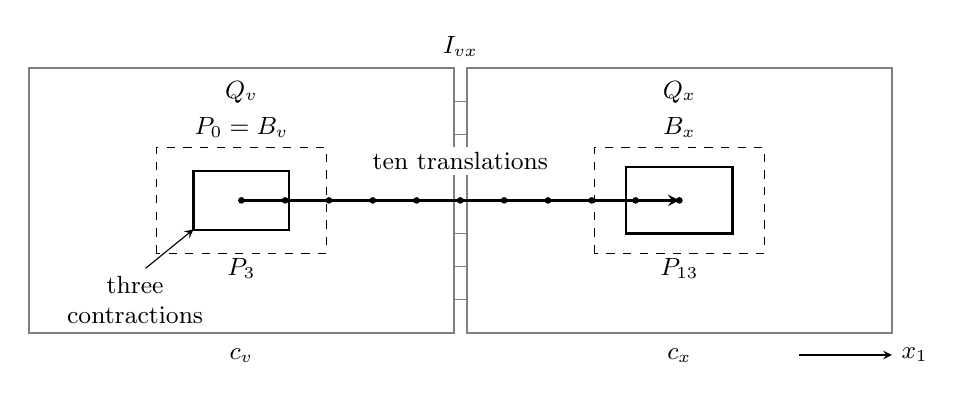
\begin{tikzpicture}[x=1.35cm,y=1.05cm,font=\small,>=stealth]
  \draw[gray,thick] (0,0) rectangle (4,3.2);
  \draw[gray,thick] (4.12,0) rectangle (8.12,3.2);
  \node at (2,2.91) {$Q_v$};
  \node at (6.12,2.91) {$Q_x$};
  \foreach \y in {0.4,0.8,1.2,1.6,2.0,2.4,2.8}{
    \draw[gray] (4,\y)--(4.12,\y);
  }
  \node[above] at (4.06,3.22) {$I_{vx}$};
  \draw[dashed] (1.2,0.96) rectangle (2.8,2.24);
  \draw[dashed] (5.32,0.96) rectangle (6.92,2.24);
  \node at (2,2.48) {$P_0=B_v$};
  \node at (6.12,2.48) {$B_x$};
  \draw[thick] (1.55,1.24) rectangle (2.45,1.96);
  \draw[thick] (5.62,1.20) rectangle (6.62,2.00);
  \node at (2,0.78) {$P_3$};
  \node at (6.12,0.78) {$P_{13}$};
  \draw[->,thick] (2,1.6)--(6.12,1.6);
  \foreach \i in {0,...,10}{
    \fill ({2+0.412*\i},1.6) circle (1.2pt);
  }
  \node[fill=white,inner sep=2pt] at (4.06,2.08) {ten translations};
  \draw[->] (1.1,0.78)--(1.55,1.25);
  \node[align=center] at (1.0,0.40) {three\\contractions};
  \node[below] at (2,-0.08) {$c_v$};
  \node[below] at (6.12,-0.08) {$c_x$};
  \draw[->] (7.25,-0.27)--(8.12,-0.27) node[right] {$x_1$};
\end{tikzpicture}
\caption{A schematic cross-section of the neighboring-box relay, not to scale.
The three contraction steps take $P_0$ to $P_3$; the marked centers then make
ten translations to $P_{13}\subset B_x$. Intermediate rectangles are omitted.
The last translation has length $2r+1$, rather than $2r$, to match the coarse
spacing $20r+1$. The narrow gap represents the interface edges between disjoint
lattice cubes, not a missing layer of lattice vertices.}
\label{geom:figure}
\end{figure}

\begin{table}[tbp]
\centering
\small
\begin{tabular}{c c c c c}
\hline
Target & Center's first coordinate & Coordinate half-widths & Radius & Normal\\
\hline
$P_1$ & $0$ & $(2r+R,4r+R,4r+R)$ & $2r$ & $1$, inward\\
$P_2$ & $0$ & $(2r+2R,2r+2R,4r+2R)$ & $2r$ & $2$, inward\\
$P_3$ & $0$ & $(2r+3R,2r+3R,2r+3R)$ & $2r$ & $3$, inward\\
$P_4$ & $2r$ & $(2r+4R)\mathbf1$ & $2r$ & $1$, forward\\
$P_5$ & $4r$ & $(2r+5R)\mathbf1$ & $2r$ & $1$, forward\\
$P_6$ & $6r$ & $(2r+6R)\mathbf1$ & $2r$ & $1$, forward\\
$P_7$ & $8r$ & $(2r+7R)\mathbf1$ & $2r$ & $1$, forward\\
$P_8$ & $10r$ & $(2r+8R)\mathbf1$ & $2r$ & $1$, forward\\
$P_9$ & $12r$ & $(2r+9R)\mathbf1$ & $2r$ & $1$, forward\\
$P_{10}$ & $14r$ & $(2r+10R)\mathbf1$ & $2r$ & $1$, forward\\
$P_{11}$ & $16r$ & $(2r+11R)\mathbf1$ & $2r$ & $1$, forward\\
$P_{12}$ & $18r$ & $(2r+12R)\mathbf1$ & $2r$ & $1$, forward\\
$P_{13}$ & $20r+1$ & $(2r+13R)\mathbf1$ & $2r+1$ & $1$, forward\\
\hline
\end{tabular}
\caption{The thirteen interfaces $P_{j-1}\to P_j$ in the relay.
All centers have second and third coordinates zero, and
$\mathbf1=(1,1,1)$. Each listed radius is used about every point
of $P_{j-1}^{(R)}$. ``Inward'' means toward zero in that normal coordinate;
``forward'' means the positive first direction. All transverse signs point
toward zero. The proof verifies both target-face and full-cube containment.}
\label{geom:interfaces}
\end{table}

\paragraph{Three contraction steps.}
For $t=1,2,3$, let $P_t$ be centered at zero with coordinate half-widths
\begin{equation}\label{geom:contraction-widths}
  a_{t,h}=\begin{cases}
    2r+tR,&h\le t,\\
    4r+tR,&h>t,
  \end{cases}
  \qquad h\in\{1,2,3\}.
\end{equation}
Fix $u\in P_{t-1}^{(R)}$. Its coordinate bounds are $2r+tR$ in directions
$h<t$ and $4r+tR$ in directions $h\ge t$. In the cube $\Lambda_{2r}(u)$,
choose a quarter-face normal to coordinate $t$, with its normal sign and both
transverse signs directed toward coordinate zero. At a zero coordinate,
either sign may be used.

In the normal direction, the face coordinate has absolute value at most
\[
  \max\{2r,(4r+tR)-2r\}=2r+tR.
\]
In a transverse direction, the face coordinate ranges between a number $a$
and $a-2r\operatorname{sign}(a)$, with either sign allowed when $a=0$.
Its absolute value is therefore at most $\max\{|a|,2r\}$, which fits the
corresponding half-width in \eqref{geom:contraction-widths}. The chosen
quarter-face is consequently contained in $P_t$.

The full cube $\Lambda_{2r}(u)$ has all coordinate absolute values at most
$6r+3R<10r$, by \eqref{geom:separation}, and so lies in $D$. In particular
$P_{t-1}^{(R)}\subseteq D$. Since $o\notin D$, the remaining geometric
hypothesis of Lemma~\ref{ext:estimate} is also satisfied. This proves its
applicability to all three contraction steps. The resulting rectangle is
\begin{equation}\label{geom:contracted}
  P_3=\Lambda_{2r+3R}(0).
\end{equation}

\paragraph{Ten translation steps.}
Define the step lengths and centers by
\begin{equation}\label{geom:translations}
  s_i=\begin{cases}2r,&1\le i\le9,\\2r+1,&i=10,\end{cases}
  \qquad
  z_0=0,\qquad z_i=(s_1+\cdots+s_i,0,0).
\end{equation}
For $1\le i\le10$, set
\begin{equation}\label{geom:translated-boxes}
  w_i=2r+(3+i)R,\qquad P_{3+i}=\Lambda_{w_i}(z_i).
\end{equation}
The $R$-expansion of the preceding rectangle, $P_{2+i}^{(R)}$, is centered
at $z_{i-1}$ and has half-width $w_i$. Fix $u$ in that expansion. In
$\Lambda_{s_i}(u)$ choose the quarter-face with forward normal in coordinate
$1$, and with both transverse signs directed toward zero. The normal
coordinate on this face is $u_1+s_i$. Relative to the new center $z_i$, its
offset is exactly $u_1-(z_{i-1})_1$, of absolute value at most $w_i$.
Transverse absolute coordinates are at most
$\max\{w_i,s_i\}=w_i$. The equality also holds for the last step, because
$13R\ge1$. Hence this quarter-face is contained in $P_{3+i}$.

To check containment of the full radius-$s_i$ cube, note that
$0\le(z_{i-1})_1\le18r$, $w_i\le2r+13R$, and $s_i\le2r+1$. Its first
coordinate is therefore between
\begin{equation}\label{geom:translation-bounds}
  -4r-13R-1\quad\hbox{and}\quad22r+13R+1,
\end{equation}
and its transverse absolute coordinates are at most $4r+13R+1$.
Condition~\eqref{geom:separation} gives $13R+1<6r$ and $13R<8r$, so these
bounds lie inside the prism \eqref{geom:prism}. It follows again that the
preceding expanded rectangle lies in $D$ and avoids $o$. The radii used
are $2r$ and $2r+1$, both allowed by Lemma~\ref{ext:estimate}. Thus all ten
translation steps satisfy that Lemma's hypotheses.

The final center is
$z_{10}=(9(2r)+(2r+1),0,0)=c_x$, and the final half-width is
$w_{10}=2r+13R<4r$. Consequently $P_{13}\subseteq B_x$. If $o$ is connected
to $P_0$ but not to $P_{13}$, then for at least one $i\in\{0,\ldots,12\}$
it is connected to $P_i$ but not to $P_{i+1}$. A union bound and thirteen
applications of Lemma~\ref{ext:estimate} now give
\[
\begin{split}
  \mathbb P\bigl(o\leftrightarrow B_v,\ o\not\leftrightarrow B_x\bigr)
  &\le
  \mathbb P\bigl(o\leftrightarrow P_0,\ o\not\leftrightarrow P_{13}\bigr)\\
  &\le \sum_{i=0}^{12}
       \mathbb P\bigl(o\leftrightarrow P_i,\ o\not\leftrightarrow P_{i+1}\bigr)
   \le 13\eta.
\end{split}
\]
No independence between these thirteen connection events is required.
\end{proof}

\section{Adaptive exploration and the final contradiction}
\label{sec:exploration}

We use the scales from Lemma~\ref{prelim:scales} to construct an infinite
open cluster at the parameter $q<p_c$. Recall the coarse cubes and their
inner boxes:
\[
 c_v=(20r+1)(v_1,v_2,0),\qquad
 Q_v=\Lambda_{10r}(c_v),\qquad B_v=\Lambda_{4r}(c_v),
 \qquad v\in\mathbb Z^2.
\]
For adjacent coarse vertices $v,x$, the interface $I_{vx}$ consists of the
lattice edges between $Q_v$ and $Q_x$. Different cubes have disjoint
vertex sets. We keep the source $o=(0,0,0)$ in the root cube $Q_0$.

\subsection{The exploration and its conditional promise}

Retaining conditional connection predictions during adaptive exploration
is the method used in Kozma and Nitzan's proof of Theorem~6
\cite[Section~4, equations~(30)--(32)]{KozmaNitzan2024}.
Here each pending cube's unknown bits are reserved until that cube is processed.

Let $\mathcal I$ be the event that all bits internal to $Q_0$ are open
and, for bonds, that all bits on its four interfaces are open. This event
has positive probability because it prescribes finitely many bits and
$q>0$. Write
\[
 \mathbb P_{\mathcal I}(\,\cdot\,)
   =\mathbb P_q(\,\cdot\mid\mathcal I).
\]
Under this law, all bits not prescribed by $\mathcal I$ are still
independent Bernoulli($q$).

Declare the coarse root good and put its four neighbors in a queue, each
with parent the root. A coarse vertex is \emph{visited} once it has been
put in the queue; the root is also visited. A queued vertex is
\emph{pending} until it is processed. Use a fixed ordering of neighbors
whenever vertices are added to the queue, and always process the first
pending vertex. No vertex is assigned a parent or queued more than once.

For each pending vertex we will retain a high conditional probability
of connection from $o$. The graph used for this prediction follows
its parent chain, so that the only bits still needed to decide the
connection will be in the pending cube and its incoming interface.
Specifically, for a pending vertex $v$, let $G(v)$ consist of the
cubes on its parent chain back to the root, all edges internal to
those cubes, and the interfaces between successive cubes of the
chain. We include no other edges, even when nonsuccessive cubes
are adjacent. Set
\[
 H_v=\{o\leftrightarrow B_v\text{ in }G(v)\}.
\]
The construction will maintain the promise
\begin{equation}
 \mathbb P_{\mathcal I}(H_v\mid\text{revealed history})>1-\delta
 \quad\text{for every pending }v.
 \label{exp:promise}
\end{equation}
A cube will acquire children only after its own connection is
verified and those children satisfy the same promise.

The invariant holds initially. For a root neighbor $v$, choose a
quarter-face of $Q_v$ facing $Q_0$. Every vertex of that quarter-face has
a neighbor in $Q_0$. By \eqref{prelim:quarterface}, the probability that
$\Lambda_m(c_v)$ connects to this quarter-face inside $Q_v$ is greater
than $1-\gamma$. Here $\Lambda_m(c_v)\subseteq B_v$. Such a connection
joins $B_v$ to $o$: the root cube and the intervening edge are open in
the bond model, while both endpoints of the intervening edge are open
in the site model. Since $\gamma<\delta$, this proves
\eqref{exp:promise} for the initial queue.

To process a pending vertex $v$, reveal the bits internal to $Q_v$ and, for
bonds, its incoming parent interface, except for bits already known.
The ancestor cubes and the interfaces joining them have been
revealed at earlier steps, so this determines $H_v$.
For each unvisited neighbor $x$ of $v$, extend $G(v)$ by $Q_x$,
its internal edges, and $I_{vx}$, obtaining a graph $G'$, and compute
\begin{equation}
 b_x=\mathbb P_{\mathcal I}
 \bigl(o\leftrightarrow B_x\text{ in }G'
       \mid\text{history after this reveal}\bigr).
 \label{exp:child-probability}
\end{equation}
The number $b_x$ is calculated from the revealed values and the
product law of the remaining bits; its computation reveals no bits.
Declare $v$ good if $H_v$ holds and $b_x>1-\delta$ for every such
neighbor. In this case, give each unvisited neighbor parent $v$
and add it to the back of the queue. Otherwise declare $v$ bad and
add no vertices. Remove $v$ from the queue in either case, and
continue until the queue is empty, if this ever occurs.

\begin{lemma}[Freshness and persistence]
\label{exp:freshness}
Conditional on any positive-probability finite revealed history, all
unrevealed bits are independent Bernoulli($q$). Moreover,
\eqref{exp:promise} holds at every step of the exploration.
\end{lemma}

\begin{proof}
The initialization fixes finitely many bits and leaves the others
independent with parameter $q$. At every later step, the preceding
revealed values determine which finite set of bits is exposed.
Conditioning on the values of this selected set again leaves the
remaining bits with their product law. The classifications, queue,
parent assignments, and numbers $b_x$ are all functions of revealed
values. They therefore add no conditions on the remaining bits.
Induction proves the first assertion.

When $x$ is assigned parent $v$, its graph $G(x)$ is precisely the
graph $G'$ used to compute $b_x$. The rule for declaring $v$ good
therefore establishes \eqref{exp:promise} for $x$ at that time.
To prove persistence, it suffices to verify that processing other
vertices cannot expose any of the unknown bits of $H_x$.

All ancestor cubes and their connecting interfaces have already
been revealed. Thus the unknown bits of $H_x$ lie in $Q_x$ or,
for bonds, on $I_{vx}$. The cubes are vertex-disjoint, so another
vertex's processing does not reveal an internal bit of $Q_x$.
Each step also reveals only the processed vertex's incoming parent
interface. Distinct parent links use distinct interfaces. Moreover, a pending
vertex has no children, since only processed good vertices acquire them.
Hence $I_{vx}$ cannot be revealed by another step while $x$ is
pending. If this interface was prescribed at initialization because
$v$ is the root, its fixed values simply remain part of the history.

Consequently, until $x$ is processed, the known bits of $H_x$ stay
fixed and its unknown bits retain the same product law. Its
conditional connection probability is unchanged. Together with the
initial verification, this proves \eqref{exp:promise} at every step.
\end{proof}

\subsection{A uniform bound on bad vertices}

\begin{lemma}
\label{exp:conditional-bad}
Immediately before any pending vertex is processed, its conditional
probability of being declared bad is less than $f$.
\end{lemma}

\begin{proof}
Condition on a positive-probability history immediately before
processing $v$. Let $\mathcal F$ denote this history and
$\mathcal F^+$ the history after the prescribed reveal at $v$.
The unvisited neighbors to be tested are already determined by
$\mathcal F$.

Fix one such neighbor $x$ and the corresponding graph $G'$. Under the
conditioning on $\mathcal F$, every bit internal to the prism
$D=Q_v\cup Q_x$ has its fresh parameter-$q$ law. To check this carefully,
neither cube has been processed: $v$ is pending and $x$ is unvisited.
Their interface has not been revealed as a parent link, since that
would require $x$ to have been visited or $v$ to have been processed.
Neither vertex is the root, so their interface is not one prescribed
by initialization. Although an initialized root interface may meet
$Q_v$, it is external to $D$. Lemma~\ref{exp:freshness} gives the
required independence.

The graph $G'$ contains every edge internal to this prism, and $o$ lies
outside it in the disjoint root cube. All exterior bits have independent
laws, with probabilities $0$ or $1$ for known bits and $q$ for unknown
bits. Thus Lemma~\ref{geom:relay} applies. If
$C_x=\{o\leftrightarrow B_x\text{ in }G'\}$, it gives
\[
 \mathbb P_{\mathcal I}(H_v\cap C_x^{\mathrm c}\mid\mathcal F)
 \le 13\eta,
\]
because $H_v$ implies a connection to $B_v$ in the larger graph $G'$.
Notice that the relay estimate is applied \emph{before} revealing
$Q_v$, not after conditioning on $H_v$.

The event $H_v$ is determined by $\mathcal F^+$, and
$b_x=\mathbb P_{\mathcal I}(C_x\mid\mathcal F^+)$. The tower property
therefore yields
\[
 \mathbb E_{\mathcal I}
   [\mathbf 1_{H_v}(1-b_x)\mid\mathcal F]\le13\eta.
\]
On $H_v\cap\{b_x\le1-\delta\}$ the integrand is at least $\delta$,
so
\[
 \mathbb P_{\mathcal I}
   (H_v\cap\{b_x\le1-\delta\}\mid\mathcal F)
 \le\frac{13\eta}{\delta}.
\]
There are at most four tests. The promise and a union bound now give
\[
 \mathbb P_{\mathcal I}(v\text{ is declared bad}\mid\mathcal F)
 \le\delta+\frac{52\eta}{\delta}<f,
\]
where the last inequality is \eqref{prelim:budgets}. No independence
between the tests is needed.
\end{proof}

\begin{lemma}
\label{exp:bad-set}
For every deterministic set of $k$ distinct coarse vertices, the
probability under $\mathbb P_{\mathcal I}$ that all are processed and
declared bad is at most $f^k$.
\end{lemma}

\begin{proof}
The assertion is immediate if the set contains the root, which is
declared good. Otherwise, fix such a set $S$. For $1\le j\le k$, let
$T_j$ be the processing time of the $j$th member of $S$ to be processed,
and set $T_j=\infty$ if fewer than $j$ members are ever processed. Let
$E_j$ be the event that $T_j<\infty$ and these first $j$ members are
all declared bad; put $E_0$ equal to the whole sample space.

For each finite time $t$, the event
\[
 \{T_j=t\}\cap E_{j-1}
\]
is determined before the reveal at time $t$. Indeed, at that moment
one knows the next vertex, how many members of $S$ have already
been processed, and whether all of those members were bad.
On $\{T_j=t\}$ there are exactly $j-1$ such previous members,
so these observations determine $E_{j-1}$ there.
After termination we keep the history constant; events specifying
a later processing time are empty. Applying
Lemma~\ref{exp:conditional-bad} at time $t$ and summing gives
\begin{align*}
 \mathbb P_{\mathcal I}(E_j)
 &\le f\sum_{t\ge1}
       \mathbb P_{\mathcal I}(T_j=t,\ E_{j-1})\\
 &\le f\,\mathbb P_{\mathcal I}(E_{j-1}).
\end{align*}
Iteration yields $\mathbb P_{\mathcal I}(E_k)\le f^k$. Since no
vertex is processed twice, $E_k$ is exactly the event in the statement.
The proof does not assume that every member of $S$ is eventually
processed.
\end{proof}

\subsection{Contours and completion of the proof}

Let $X$ be the set of good coarse vertices, including the root. If $X$
is finite, only finitely many vertices can ever enter the queue: new
entries arise only from good vertices, with at most four per vertex.
The queue must therefore empty after finitely many steps. Every vertex
outside $X$ adjacent to $X$ has then been processed and declared bad.
Indeed, the root's neighbors were all queued at initialization. When
any nonroot good vertex was processed, each of its neighbors was either
already visited or assigned at that step. Thus every outside neighbor
of $X$ is processed before termination and is not good, so it is bad.

Apply Lemma~\ref{prelim:contours} to this finite set $X$, which contains
the origin of the coarse lattice. Its boundary contains a cycle of
some length $n$ in the deterministic family of at most $2n3^n$
candidates. For each candidate, fix the matching of crossed primal
edges supplied by that Lemma. It has $k\ge n/7$ edges with pairwise
disjoint endpoints. If the candidate occurs as a boundary cycle of
$X$, every one of these edges has a bad endpoint outside $X$.

For a fixed candidate there are $2^k$ ways to choose one endpoint from
each matching edge. Each choice is a deterministic set of $k$ distinct
vertices, so Lemma~\ref{exp:bad-set} bounds the probability that all
chosen vertices are processed bad by $f^k$. Hence the candidate's
probability is at most
\[
 2^k f^k=(2f)^k\le(2f)^{n/7},
\]
using $2f<1$. We have not conditioned on the random set $X$ or on the
occurrence of a cycle. Taking the union bound over the deterministic
candidate families and using the choice of $f$ in
Lemma~\ref{prelim:scales} gives
\begin{equation}
 \mathbb P_{\mathcal I}(|X|<\infty)
 \le\sum_{n\ge1}2n3^n(2f)^{n/7}<1.
 \label{exp:infinite-good}
\end{equation}

Thus, with positive probability under $\mathbb P_{\mathcal I}$,
infinitely many coarse vertices are good. Every good nonroot vertex
$v$ satisfies the actual connection event $H_v$. The boxes $B_v$ are
pairwise disjoint, so these connections put infinitely many lattice
vertices in the open cluster of $o$. Therefore
\[
 \mathbb P_q(o\text{ belongs to an infinite open cluster})
 \ge \mathbb P_q(\mathcal I)\,
       \mathbb P_{\mathcal I}(|X|=\infty)>0.
\]
This contradicts $q<p_c$. The assumption of critical percolation was
therefore false. The construction and all its estimates apply to
both bond and site percolation with their respective critical
parameters, proving Theorem~\ref{thm:main}.

The finite computations are not formal proof certificates.

\begin{thebibliography}{99}
\raggedright

\bibitem{BenjaminiSchramm1996}
Itai Benjamini and Oded Schramm.
Percolation beyond $\mathbb Z^d$, many questions and a few answers.
\emph{Electronic Communications in Probability} \textbf{1} (1996), 71--82.
\href{https://doi.org/10.1214/ECP.v1-978}{doi:10.1214/ECP.v1-978}.

\bibitem{BroadbentHammersley1957}
S.~R. Broadbent and J.~M. Hammersley.
Percolation processes. I. Crystals and mazes.
\emph{Proceedings of the Cambridge Philosophical Society}
\textbf{53} (1957), no.~3, 629--641.
\href{https://doi.org/10.1017/S0305004100032680}{doi:10.1017/S0305004100032680}.

\bibitem{SitePublic2026}
ChatGPT 5.6, prompted by Ahmed Bou-Rabee;
exposition and formalization support by Claude Opus 5 and GLM 5.3.
\emph{Percolation at criticality}.
Public research exposition, updated September 5, 2026.
\href{https://nitromannitol.github.io/site-percolation-7d3f2/}{Public exposition}.

\bibitem{KNPublic2026}
ChatGPT 5.6 Sol and Claude Fable 5.1, prompted by Ahmed Bou-Rabee.
\emph{Kozma--Nitzan inequalities: proofs and counterexamples}.
Public research exposition, updated September 5, 2026.
\href{https://nitromannitol.github.io/kn1-verification-b80e9/}{Public exposition}.

\bibitem{DuminilCopinSidoraviciusTassion2016}
Hugo Duminil-Copin, Vladas Sidoravicius, and Vincent Tassion.
Absence of infinite cluster for critical Bernoulli percolation on slabs.
\emph{Communications on Pure and Applied Mathematics}
\textbf{69} (2016), no.~7, 1397--1411.
\href{https://doi.org/10.1002/cpa.21641}{doi:10.1002/cpa.21641}.

\bibitem{FitznerHofstad2017}
Robert Fitzner and Remco van der Hofstad.
Mean-field behavior for nearest-neighbor percolation in $d>10$.
\emph{Electronic Journal of Probability} \textbf{22} (2017), paper no.~43, 1--65.
\href{https://doi.org/10.1214/17-EJP56}{doi:10.1214/17-EJP56}.

\bibitem{GrimmettMarstrand1990}
G.~R. Grimmett and J.~M. Marstrand.
The supercritical phase of percolation is well behaved.
\emph{Proceedings of the Royal Society of London. Series A}
\textbf{430} (1990), no.~1879, 439--457.
\href{https://doi.org/10.1098/rspa.1990.0100}{doi:10.1098/rspa.1990.0100}.

\bibitem{HaraSlade1990}
Takashi Hara and Gordon Slade.
Mean-field critical behaviour for percolation in high dimensions.
\emph{Communications in Mathematical Physics}
\textbf{128} (1990), no.~2, 333--391.
\href{https://doi.org/10.1007/BF02108785}{doi:10.1007/BF02108785}.

\bibitem{Harris1960}
Theodore E. Harris.
A lower bound for the critical probability in a certain percolation process.
\emph{Proceedings of the Cambridge Philosophical Society}
\textbf{56} (1960), no.~1, 13--20.
\href{https://doi.org/10.1017/S0305004100034241}{doi:10.1017/S0305004100034241}.

\bibitem{HeydenreichMatzke2020}
Markus Heydenreich and Kilian Matzke.
Critical site percolation in high dimension.
\emph{Journal of Statistical Physics} \textbf{181} (2020), 816--853.
\href{https://doi.org/10.1007/s10955-020-02607-y}{doi:10.1007/s10955-020-02607-y}.

\bibitem{Kesten1980}
Harry Kesten.
The critical probability of bond percolation on the square lattice equals $1/2$.
\emph{Communications in Mathematical Physics} \textbf{74} (1980), 41--59.
\href{https://doi.org/10.1007/BF01197577}{doi:10.1007/BF01197577}.

\bibitem{KozmaNitzan2024}
Gady Kozma and Shahaf Nitzan.
A reduction of the $\theta(p_c)=0$ problem to a conjectured inequality.
Preprint, 2024.
\href{https://arxiv.org/abs/2401.12397v1}{arXiv:2401.12397v1}.

\bibitem{Leder2026}
Justin Leder.
\emph{$\theta(p_c)=0$ for Bernoulli bond percolation on $\mathbb Z^d$
in all dimensions $d\ge2$: a guide to the Lean formalization}.
Public research announcement, August 2026.
\href{https://github.com/anthropics/formal-math/blob/795efb86f191735c5481675763537cfb4ff37e55/percolation/summary.pdf}{Pinned repository version},
commit \texttt{795efb86f191}.

\bibitem{Russo1981}
Lucio Russo.
On the critical percolation probabilities.
\emph{Zeitschrift f\"ur Wahrscheinlichkeitstheorie und verwandte Gebiete}
\textbf{56} (1981), no.~2, 229--237.
\href{https://doi.org/10.1007/BF00535742}{doi:10.1007/BF00535742}.

\bibitem{BHK2006}
J.~van den Berg, O.~H\"aggstr\"om, and J.~Kahn.
Some conditional correlation inequalities for percolation and related processes.
\emph{Random Structures \& Algorithms} \textbf{29} (2006), no.~4, 417--435.
\href{https://doi.org/10.1002/rsa.20102}{doi:10.1002/rsa.20102}.

\end{thebibliography}

\end{document}
